\section{Implementação}
\label{sec:implementacao}

Esta seção descreve a implementação do ValorizeAI, enfatizando os elementos arquiteturais, os fluxos de execução e os componentes que foram exercitados nos experimentos de carga. O objetivo é apresentar como o sistema opera internamente, de modo a contextualizar os resultados apresentados na próxima seção.

\subsection{Arquitetura Lógica da Aplicação}

A aplicação segue uma arquitetura modular composta por três subsistemas principais:

\begin{itemize}
    \item \textbf{Serviço HTTP (API Laravel):} responsável pelas operações transacionais síncronas (consultas, criação de transações, ingestão de dados e automações).
    \item \textbf{Servidor WebSocket (Laravel Reverb):} dedicado ao envio de notificações em tempo real e atualização dos dashboards.
    \item \textbf{Workers HTTP (Cloud Run):} executores de tarefas assíncronas disparadas pelo Cloud Tasks.
\end{itemize}

Cada subsistema é implantado como serviço independente no Cloud Run, permitindo escalonamento isolado e controle fino de concorrência.

\subsection{Fluxo Síncrono: API HTTP}

O backend Laravel organiza o domínio financeiro em módulos que seguem Clean Architecture e DDD. As rotas públicas acessam controladores que delegam:

\begin{itemize}
    \item \textbf{consultas} para classes \textit{Query}, otimizadas para leitura e usando Redis como cache;
    \item \textbf{escritas} para classes \textit{Action}, que encapsulam validações, regras de negócio, transações no PostgreSQL e emissão de eventos.
\end{itemize}

Os endpoints exercitados nos testes k6 incluem:

\begin{itemize}
    \item \verb|GET /api/transactions|, leitura intensiva de listas paginadas;
    \item \verb|POST /api/transactions|, criação de transações, fluxo que ativa lógica de consistência e atualizações derivadas;
    \item \verb|GET /api/accounts|, consulta leve usada para refletir mudanças de saldo.
\end{itemize}

O caminho de leitura foi otimizado com cache \textit{cache-aside}: a primeira consulta popula Redis, e subsequentes retornam em baixa latência.
O caminho de escrita, por sua vez, não usa cache e realiza operações ACID no PostgreSQL.
Esse fluxo é ilustrado na Figura~\ref{fig:fluxo-sincrono}.

\begin{figure}[htbp]
    \centering
    \begin{tikzpicture}[
        node distance=0.9cm and 1.8cm,
        >=Latex,
        box/.style={
            draw,
            rounded corners,
            align=center,
            minimum width=3.4cm,
            minimum height=0.9cm,
            font=\footnotesize
        }
    ]
        % Linha principal
        \node[box] (client) {Cliente / gerador de carga (k6)};
        \node[box, below=of client] (controller) {Controladores HTTP\\(Laravel)};

        % Split Query / Action
        \node[box, below left=of controller]  (query)  {Camada de leitura\\(\textit{Query})};
        \node[box, below right=of controller] (action) {Camada de escrita\\(\textit{Action})};

        % Armazenamento
        \node[box, below=of query]  (redis) {Redis (cache)};
        \node[box, below=of action] (pg)    {PostgreSQL (ACID)};

        % Setas principais
        \draw[->] (client) -- node[right]{HTTP} (controller);
        \draw[->] (controller) -- node[left]{consultas} (query);
        \draw[->] (controller) -- node[right]{escritas} (action);

        % Leitura: cache-aside
        \draw[->] (query) -- node[left]{consulta / cache-aside} (redis);
        \draw[->] (query) -- node[right]{leitura} (pg);

        % Escrita: só banco
        \draw[->] (action) -- node[right]{transações ACID} (pg);
    \end{tikzpicture}
    \caption{Fluxo síncrono da API HTTP, destacando a separação entre caminhos de leitura (\textit{Query} + Redis) e escrita (\textit{Action} + PostgreSQL).}
    \label{fig:fluxo-sincrono}
\end{figure}


\subsection{Fluxo Assíncrono: Cloud Tasks e Workers}

Tarefas que exigem maior tempo de processamento são delegadas ao pipeline assíncrono. O processo ocorre em quatro etapas:

\begin{enumerate}
    \item a API cria uma tarefa via Cloud Tasks, anexando o payload necessário;
    \item o serviço envia uma requisição HTTP \textit{push} para o endpoint do worker;
    \item o Cloud Run instancia dinamicamente quantos workers forem necessários para consumir o backlog;
    \item cada worker executa o processamento (ex.: importação de extratos, geração de relatórios, triggers de automações).
\end{enumerate}

O uso de \textit{push queues} elimina a necessidade de processos consumidores contínuos e garante elasticidade automática baseada no ritmo de produção.

Esse fluxo é ilustrado na Figura~\ref{fig:fluxo-assincrono}.

\begin{figure}[htbp]
    \centering
    \begin{tikzpicture}[
        node distance=0.9cm,
        >=Latex,
        box/.style={
            draw,
            rounded corners,
            align=center,
            minimum width=3.4cm,
            minimum height=0.9cm,
            font=\footnotesize
        }
    ]
        % Coluna vertical
        \node[box] (client) {Cliente / gerador de carga (k6)};
        \node[box, below=of client] (api) {API HTTP\\(Cloud Run + Laravel)};
        \node[box, below=of api] (tasks) {Cloud Tasks\\(fila HTTP \emph{push})};
        \node[box, below=of tasks] (worker) {Workers HTTP\\(Cloud Run)};
        \node[box, below=of worker] (db) {PostgreSQL / Redis};

        % Setas
        \draw[->] (client) -- node[right]{HTTP} (api);
        \draw[->] (api) -- node[right]{Criação de tarefas} (tasks);
        \draw[->] (tasks) -- node[right]{Entrega \emph{push}} (worker);
        \draw[->] (worker) -- node[right]{Processamento ACID / eventos} (db);
    \end{tikzpicture}
    \caption{Fluxo assíncrono entre API HTTP, Cloud Tasks e workers em Cloud Run.}
    \label{fig:fluxo-assincrono}
\end{figure}

\subsection{Comunicação em Tempo Real: WebSockets com Reverb e Redis}

O servidor WebSocket do Reverb mantém conexões persistentes com os clientes do painel em tempo real. Como o ambiente Cloud Run escala horizontalmente e instancia múltiplos contêineres, cada instância possui um conjunto próprio de clientes conectados.

Para distribuir eventos entre elas, utiliza-se Redis como \textit{backplane} Pub/Sub:

\begin{itemize}
    \item Instâncias publicam eventos em canais Redis.
    \item Todas as instâncias inscritas recebem as mensagens.
    \item A instância que possui o cliente conectado retransmite o evento via WebSocket.
\end{itemize}

Esse mecanismo assegura coerência e funcionamento correto mesmo em ambientes altamente elásticos.

A Figura~\ref{fig:reverb-redis} resume a relação entre instâncias do Reverb, Redis e clientes conectados

\begin{figure}[htbp]
    \centering
    \begin{tikzpicture}[
        node distance=0.9cm and 2.0cm,
        >=Latex,
        box/.style={
            draw,
            rounded corners,
            align=center,
            minimum width=3.4cm,
            minimum height=0.9cm,
            font=\footnotesize
        }
    ]
        % Camada superior: produtores de eventos
        \node[box] (api) {API HTTP / Workers};
        % \node[box, right=of api] (worker) {Workers HTTP};

        % Redis central (abaixo da API, mais ou menos no meio)
        \node[box, below=of api] (redis) {Redis (Pub/Sub)};

        % Reverb logo abaixo do Redis
        \node[box, below left=of redis]  (reverbA) {Reverb -- instância A};
        \node[box, below right=of redis] (reverbB) {Reverb -- instância B};

        % Clientes conectados
        \node[box, below=of reverbA] (client1) {Clientes conectados};
        \node[box, below=of reverbB] (client2) {Clientes conectados};

        % Setas de eventos da aplicação para o Redis
        \draw[->] (api) -- node[left]{Eventos} (redis);
        % \draw[->] (worker) |- node[right]{Eventos} (redis);

        % Pub/Sub entre Redis e Reverb
        \draw[<->] (redis) -- node[left]{Pub/Sub} (reverbA);
        \draw[<->] (redis) -- node[right]{Pub/Sub} (reverbB);

        % WebSockets para os clientes
        \draw[<->] (reverbA) -- node[left]{WebSocket} (client1);
        \draw[<->] (reverbB) -- node[right]{WebSocket} (client2);
    \end{tikzpicture}
    \caption{Distribuição de eventos em tempo real via Redis e instâncias do servidor WebSocket Reverb.}
    \label{fig:reverb-redis}
\end{figure}

\FloatBarrier
\subsection{Modelo de Dados e Otimizações}

O modelo lógico (Figura~\ref{fig:modelo-dados}) segue um desenho multi-inquilino composto por usuários, contas, categorias e orçamentos que representam a estrutura organizacional do sistema, além de transações e divisões (\textit{splits}) responsáveis por manter a granularidade das movimentações financeiras. Embeddings vetoriais, armazenados via \texttt{pgvector}, complementam o modelo ao fornecer suporte para classificação automática e comparação semântica de registros, justificando sua presença mesmo em um ambiente relacional tradicional.

\begin{figure}[H]
    \centering
    \resizebox{0.95\linewidth}{!}{%
    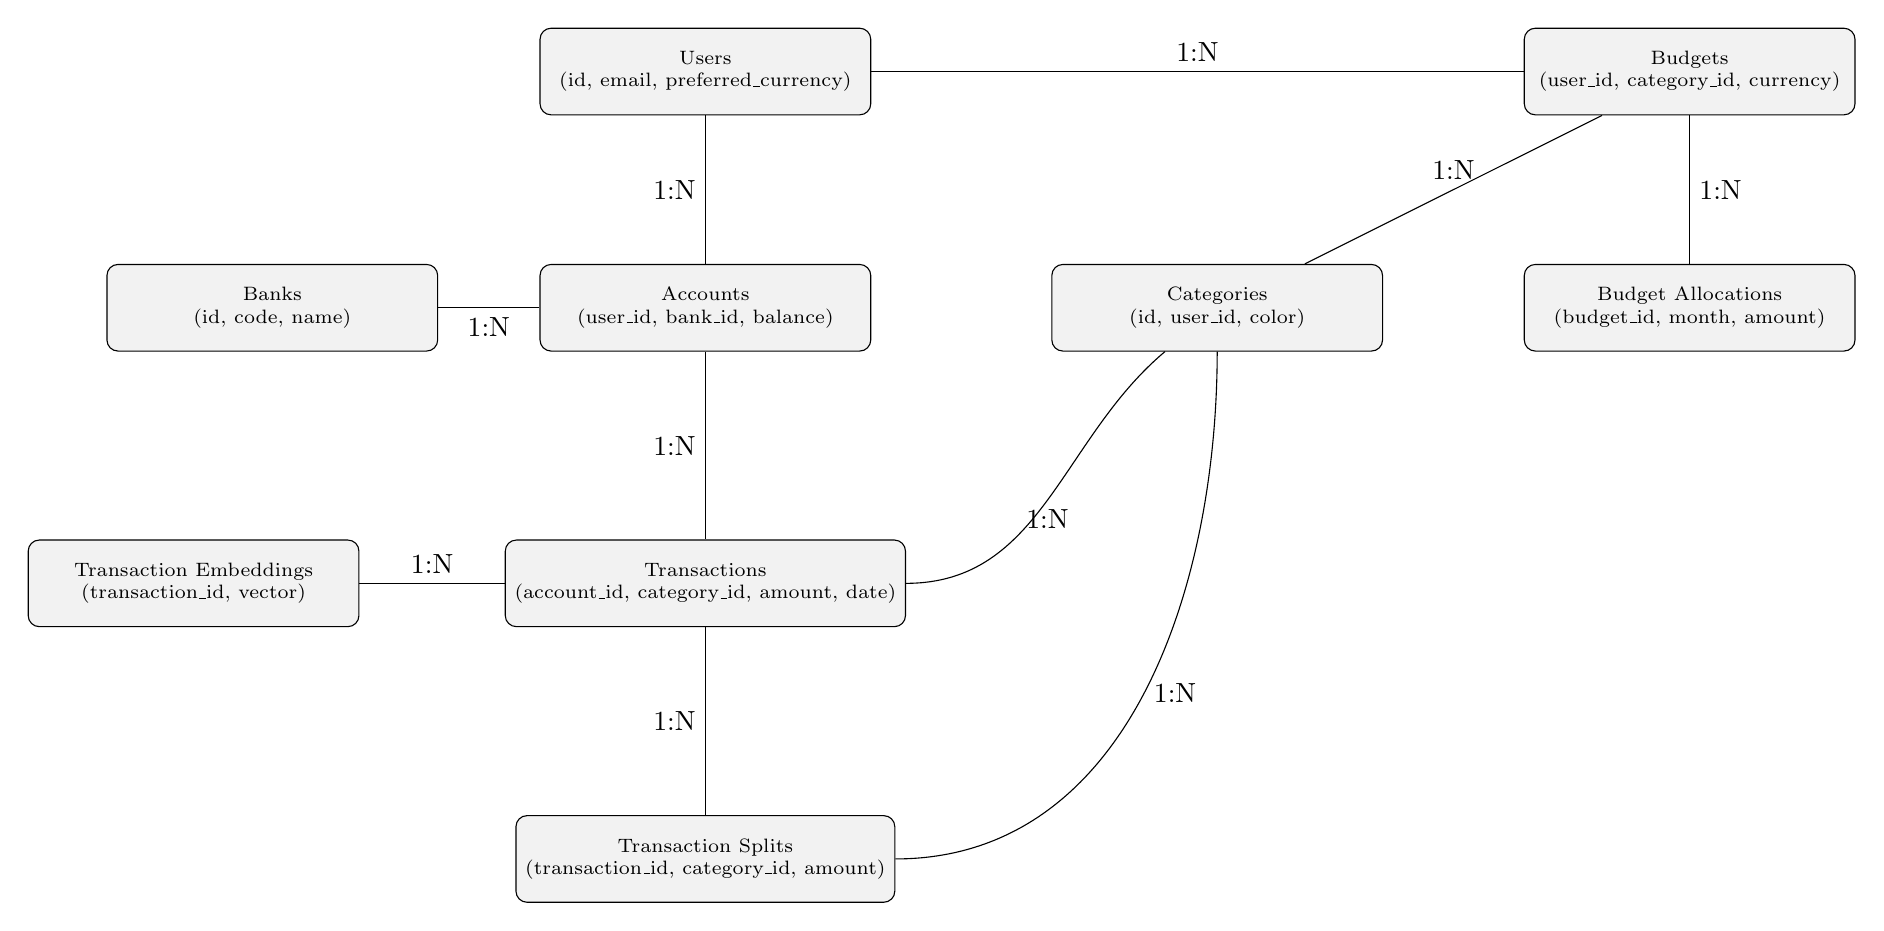
\begin{tikzpicture}[
        table/.style={draw, rounded corners, fill=gray!10, minimum width=4.2cm, minimum height=1.1cm, font=\scriptsize, align=center},
        every edge/.style={->, very thick, >=Stealth}
    ]
        \node (users) at (0,1.5) [table] {Users\\(id, email, preferred\_currency)};
        \node (banks) at (-5.5,-1.5) [table] {Banks\\(id, code, name)};
        \node (accounts) at (0,-1.5) [table] {Accounts\\(user\_id, bank\_id, balance)};
        \node (transactions) at (0,-5.0) [table] {Transactions\\(account\_id, category\_id, amount, date)};
        \node (splits) at (0,-8.5) [table] {Transaction Splits\\(transaction\_id, category\_id, amount)};

        \node (categories) at (6.5,-1.5) [table] {Categories\\(id, user\_id, color)};
        \node (embeddings) at (-6.5,-5.0) [table] {Transaction Embeddings\\(transaction\_id, vector)};
        \node (budgets) at (12.5,1.5) [table] {Budgets\\(user\_id, category\_id, currency)};
        \node (allocations) at (12.5,-1.5) [table] {Budget Allocations\\(budget\_id, month, amount)};

        \draw (users) -- node[midway,left]{1:N} (accounts);
        \draw (banks) -- node[midway,below]{1:N} (accounts);
        \draw (accounts) -- node[midway,left]{1:N} (transactions);
        \draw (transactions) -- node[midway,left]{1:N} (splits);
        \draw (transactions) -- node[midway,above]{1:N} (embeddings);

        \draw (users) -- node[midway,above]{1:N} (budgets);
        \draw (categories) -- node[midway,above]{1:N} (budgets);
        \draw (budgets) -- node[midway,right]{1:N} (allocations);

        \draw (categories) to[out=-140,in=0] node[midway,below]{1:N} (transactions);
        \draw (categories) to[out=-90,in=0] node[midway,right]{1:N} (splits);
    \end{tikzpicture}}
    \caption{Modelo lógico central derivado do esquema relacional do ValorizeAI.}
    \label{fig:modelo-dados}
\end{figure}

Para sustentar o volume de leituras e escritas observado, foram aplicadas otimizações específicas. Índices compostos em \verb|transactions(date, account_id)| aceleram filtros combinados por data e conta, enquanto a padronização da paginação reduz o fan-out em cenários com alto paralelismo. A projeção de DTOs limita a transferência de dados apenas ao necessário para o front-end, preservando largura de banda e diminuindo o trabalho de serialização. Por fim, o pré-aquecimento da cache com consultas frequentes garante que o Redis já contenha os conjuntos de dados mais requisitados antes dos testes, minimizando latência inicial e variações entre execuções.

\subsection{Observabilidade e Instrumentação}

A coleta de evidências envolveu um conjunto integrado de ferramentas. O \textbf{Cloud Monitoring} forneceu métricas de CPU, memória, instâncias ativas, latência e backlog do Cloud Tasks, permitindo enxergar a reação da infraestrutura conforme as cargas variavam. Os \textbf{CSVs automatizados do k6} serviram como fonte canônica para SLIs de latência e taxa de erro, garantindo comparabilidade entre execuções. \textbf{Logs estruturados} foram emitidos para cada requisição crítica a fim de rastrear saturação do banco e falhas de escrita, enquanto \textbf{dashboards personalizados} consolidaram esses dados para acompanhar em tempo real o comportamento dos serviços do Cloud Run durante os experimentos. Essa infraestrutura correlaciona aplicação, banco, Redis, filas e WebSockets com precisão suficiente para justificar as conclusões da Seção~\ref{sec:resultados}.

\subsection{Síntese da Implementação}

A integração entre API síncrona, pipeline assíncrono via Cloud Tasks, cache Redis e servidor WebSocket escalável fornece a base operacional necessária para avaliar os SLOs definidos. O comportamento observado sob tráfego elevado é consequência direta dessas decisões: a API concentra o domínio e delega trabalho pesado aos workers, o Redis mantém leituras rápidas e sincroniza eventos em tempo real, e o Reverb garante que notificações persistam mesmo com escalonamento horizontal. Juntos, esses componentes amarram as otimizações descritas ao longo da seção e sustentam os experimentos discutidos posteriormente.
